
% this file is called up by thesis.tex
% content in this file will be fed into the main document

% ----------------------- introduction file header -----------------------
\chapter{The Trigger system upgrade for High-Luminosity LHC}
\label{chapter:upgrade}
% ----------------------- paths to graphics ------------------------

% the code below specifies where the figures are stored
\graphicspath{Chapters/CH3/figures}

% ----------------------------------------------------------------------
% ----------------------- introduction content -------------------------
% ----------------------------------------------------------------------
Since the beginning, the LHC accelerator has faced operating periods and dedicated shut-downs to
upgrade the accelerator machine and the detectors. In Figure~\ref{fig:phase2} a summary of the LHC timeline for operation and upgrade is shown.
\begin{figure}[!h]
	\centering
	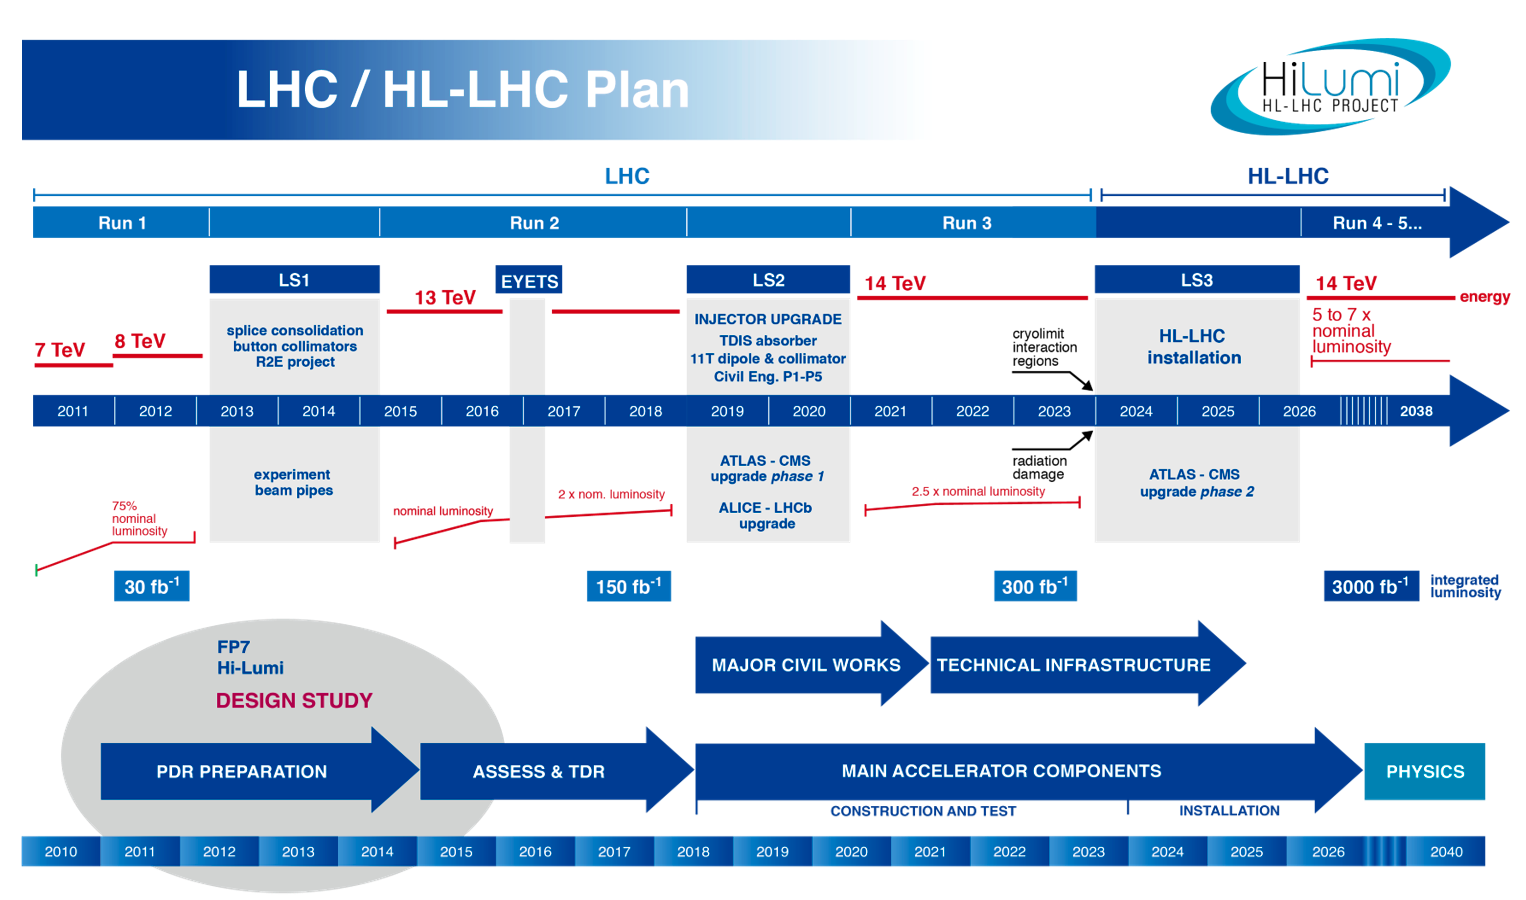
\includegraphics[width=0.9\textwidth]{Chapters/CH3/figures/phase2}
	\caption{Summary of the LHC timeline for operation and upgrade~\cite{phase2}.}
	\label{fig:phase2}
\end{figure}
\\At the end of 2018, the LHC was shut-down and for two years it will be upgraded to reach the center-of-mass energy to its design value of 14 TeV and collect 300 $\mathrm{fb^{-1}}$ of data, almost double of the current available statistics of Run2.\\
After 4 years of duty cycle, the High-Luminosity period of LHC (HL-LHC) will start and aims to bring the integrated luminosity to 3000 $\mathrm{fb^{-1}}$, unlocking several studies, mostly related with rare phenomena, which are impossible to perform with the curreent statistics.\\
The main focus of this chapter is the trigger system upgrade for HL-LHC and several studies will be presented.

\section{ATLAS Barrel Muon Trigger}
The muon detector chambers are arranged such that particles from the interaction point traverse three stations of chambers.\\
The system is subdivided azimuthally into 16 sectors numbered from 1 to 16.
The sector number increases in the direction of increasing $\mathrm{\phi}$ with the number 1 corresponding to coordinate $\mathrm{\phi=0}$. The odd sector (called “large sectors”)
are located between barrel coils, instead, the even sectors (called “small sectors”) are covered by the coils.\\
The muon spectrometer consists of three large air-core superconducting toroidal magnets (two end-caps and one barrel) providing a field of approximately 0.5 T.\\
In the barrel, the chambers are arranged in three concentric cylinders around the beam axis called BI (Barrel Inner), BM (Barrel Middle), and BO (Barrel Outer). \\
RPC planes are installed in the Middle
and Outer stations of the Muon Spectrometer always mechanically associated with MDT precision chambers (except for some “special” chambers). \\
Two RPC planes are integrated with MDT in the Middle stations and one RPC plane only in the Outer stations.\\
Schematic drawings of the present ATLAS MS~\cite{TDR}, are shown in Figures~\ref{fig:MS_rz} and~\ref{fig:MS_xy2}.
\begin{figure}[!h]
	\centering
	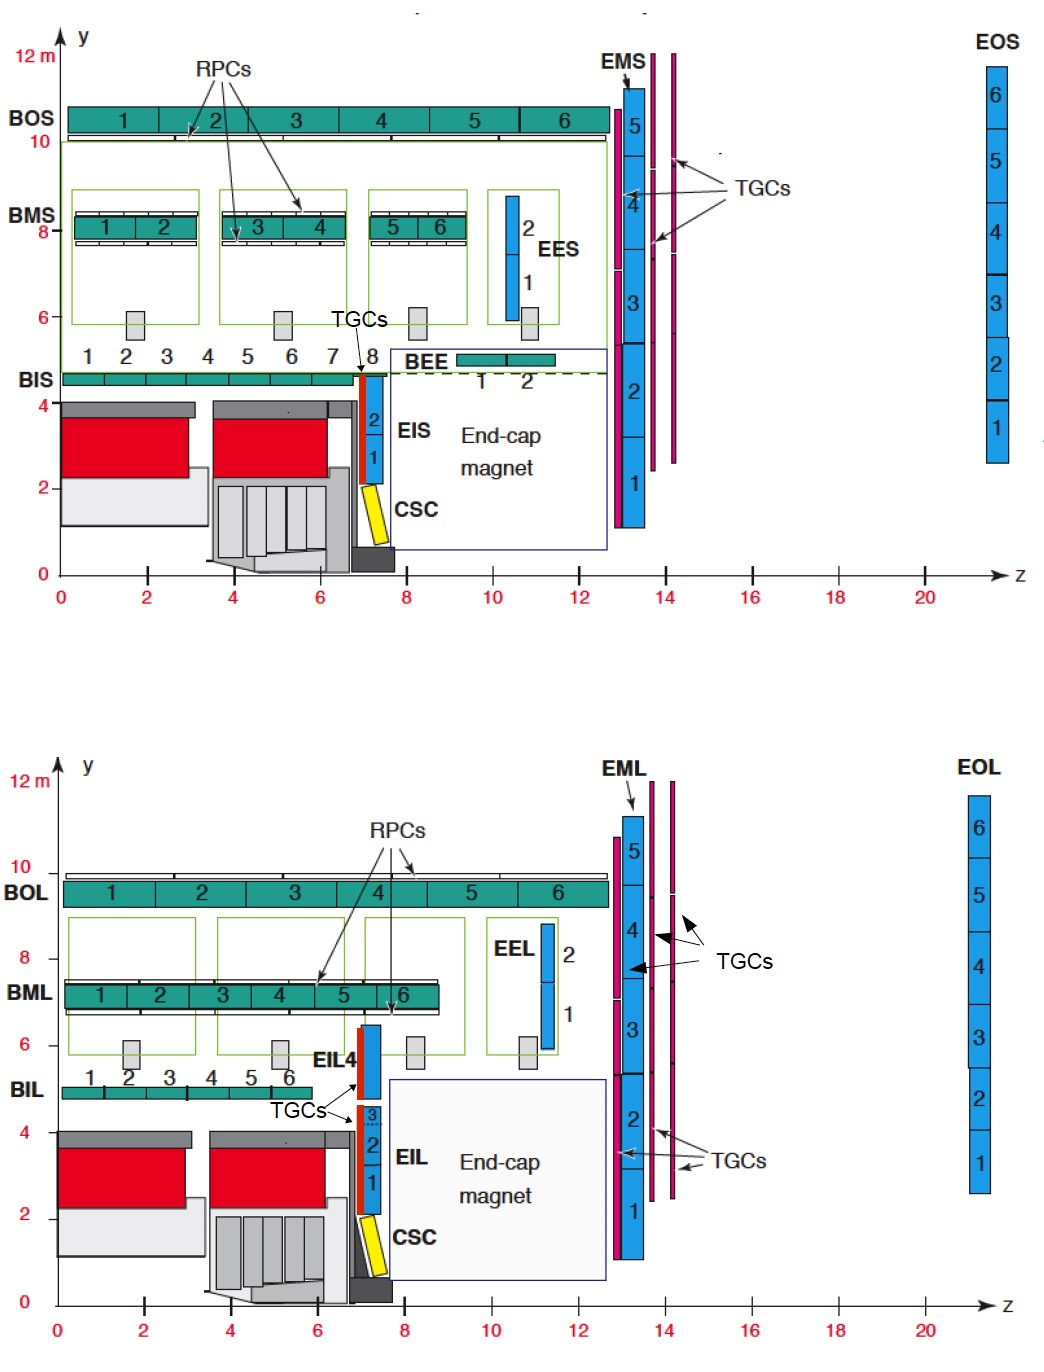
\includegraphics[width=0.9\textwidth]{Chapters/CH3/figures/MS_rz}
	\caption{Two R-Z views of of the present (Run 1/2) ATLAS muon spectrometer layout. Top: One of the azimuthal sectors that contain the barrel toroid coils (small sector). Bottom: One of the sectors in-between the barrel toroid coils (large sector)~\cite{TDR}.}
	\label{fig:MS_rz}
\end{figure}
\begin{figure}[!h]
	\centering
	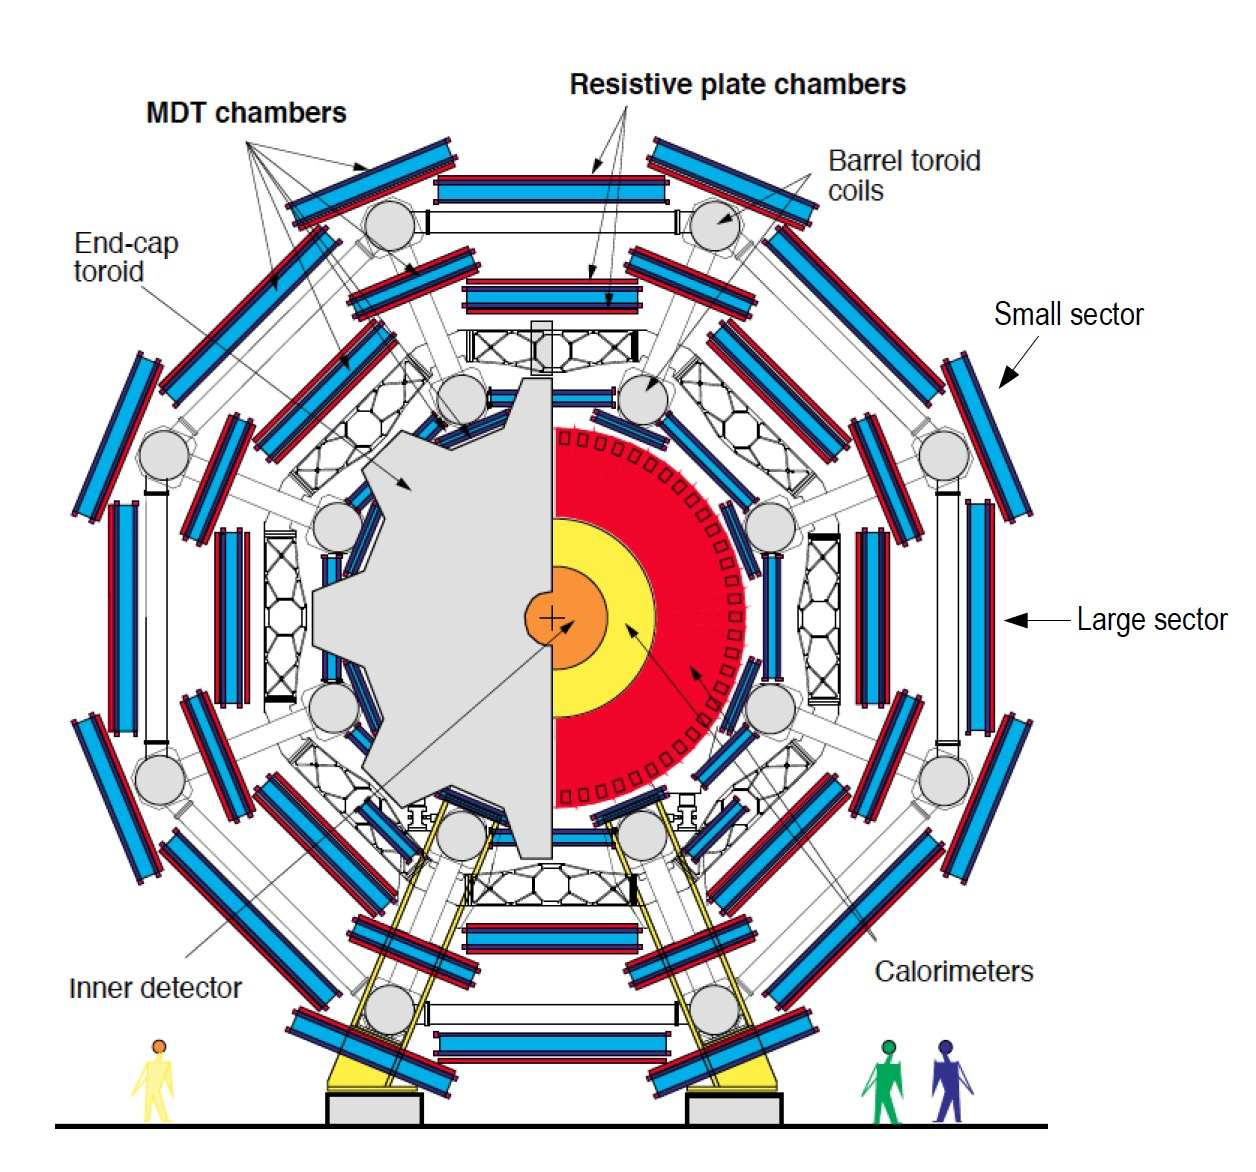
\includegraphics[width=0.9\textwidth]{Chapters/CH3/figures/MS_xy}
	\caption{View of the present (Run 1/2) ATLAS muon spectrometer barrel layout in the plane transverse to the beam axis (X-Y plane)~\cite{TDR}.}
	\label{fig:MS_xy2}
\end{figure}
The MS detector and electronics components have been designed for 10 years of operation
at a luminosity of $\mathrm{1\times 10^{34}cm^{-2} s^{-1}}$, corresponding to an integrated luminosity of $\mathrm{1000 fb^{-1}}$. 
Conservative safety factors for radiation tolerance and rate capability were taken
into account in the original designs, and components have been tested up to and above
levels corresponding to the expected doses and rates predicted by simulations multiplied
by the safety factors. After the start of LHC operation, detector hit rates and radiation doses
could be measured directly, and the previous simulations have been found to agree with
the measurements to within a maximum deviation of about 50$\%$.
\\Based on this observation, the original safety factors were reduced [10], and as a consequence the original irradiation and high-rate tests have qualified the detectors for longer running and higher rates than originally anticipated.


\section {BI upgrade for Phase II}
In the Phase-I upgrade, foreseen for LS2, the Small Wheels will be replaced by the New Small Wheels (NSW)~\cite{NSW} using small-strip TGC (sTGC) and Micro-Mesh Gaseous Structure
(MicroMeGaS or Micromegas, MM for short) chambers used for both triggering and precision tracking.\\
At the time of the Phase-II upgrade, there will thus be no CSC chambers
any more in the detector, nor will there be the Small Wheel MDT chambers, which are the ones closest to the beam line and exposed to the highest rates. Also in LS2, the BIS7 and
BIS8 MDT chambers will be replaced by integrated BIS78 stations of new RPC and small diameter MDT (sMDT) chambers to enhance the trigger coverage in this region ~\cite{BIS78}.\\
Schematic drawings of the ATLAS MS with the new detectors that will be installed in the Phase-I and Phase-II upgrades are shown in Figure~\ref{fig:MS_rz_update}.\\
\begin{figure}
	\centering
	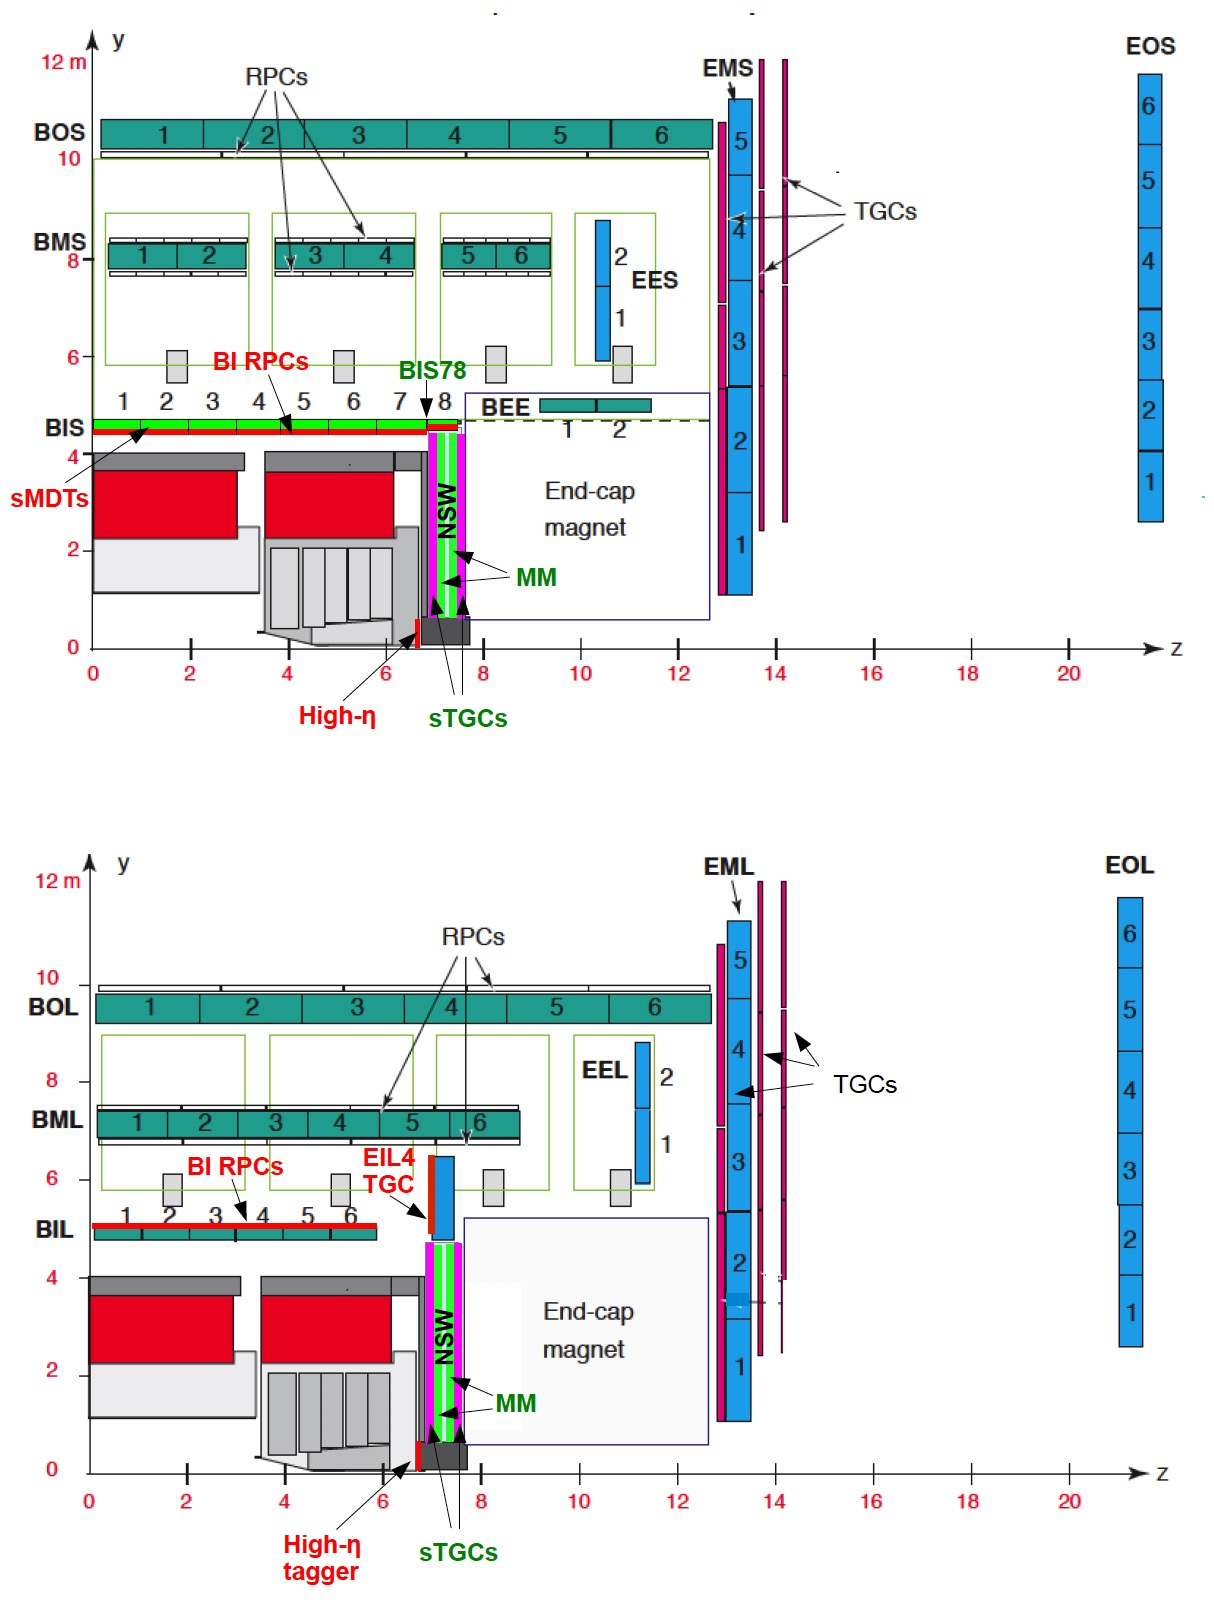
\includegraphics[width=0.9\textwidth]{Chapters/CH3/figures/MS_rz_update}
	\caption{Two R-Z views of the Phase-II ATLAS muon spectrometer layout showing a small sector (top) and a large sector (bottom). The drawings show the new detectors to be added in the Phase-II upgrade, including the addition of the high-$\mathrm{\eta}$ tagger (red text: BI RPC, sMDT, EIL4 TGC, high-$\mathrm{\eta}$ tagger), those to be installed during LS2 (green text: Micromegas and sTGC in the New Small Wheel and BIS78 RPC and sMDT), and those that will remain unchanged from the Run 1 layout (black text)~\cite{TDR}.}
	\label{fig:MS_rz_update}
\end{figure}

\noindent To maintain a high trigger efficiency, new RPC chambers with increased rate capability will be installed on the inner (BI) MDT chambers of the barrel. This addresses a fundamental issue
of the present (old) RPC chambers: to ensure their continued operation at the HL-LHC,
these chambers will have to be operated at reduced performance (i.e. efficiency), in order to
respect the original design limits on currents and integrated charge. This can be achieved
by reducing the gas gain through lowering the operating voltages. In the areas of highest
backgrounds, the gas gain will have to be reduced to such low levels that hit inefficiencies
up to 35$\%$ will be encountered. This would reduce the trigger efficiency in the barrel region
to an unacceptable level if no compensating measures were taken. In addition, due
to changes in regulations, the present gas mixture used in ATLAS RPCs may need to be
replaced by one with lower global-warming potential (GWP). Unless new gas mixtures are
found in time, this too will imply operation of old RPCs at a reduced efficiency. Despite
the lower single-hit efficiencies, a high trigger efficiency and purity can be maintained by
loosening the requirements on hit coincidences in the old chambers, if at the same time a
coincidence with the new BI RPC chambers is introduced. The installation of these chambers
will also close most of the acceptance holes of the present barrel muon trigger, which
amount to more than 20$\%$ of the $\eta-\phi$ coverage for $\eta$ < 1.05.\\

\noindent Adding new RPC chambers in the barrel is challenging in terms of available space and
installation. In the small sectors, the BI RPC chambers can only be installed if the present
MDT chambers are replaced by new sMDT chambers with reduced overall thickness so that
the sMDT chambers and the new RPCs fit in the same envelope as the original MDT chambers.
In the large sectors there is sufficient space available to add the new RPC chambers
without replacing the MDTs, if on-detector services are re-arranged.\\
The retrofitting of selected RPC chambers in the BM and BO layer in the areas of highest
rate at $\eta$ > 0.8, namely the BML7 and BOL6 chambers, is a small additional upgrade. The
MDT+RPC stations will be temporarily removed from the detector to replace the front-end
electronics and the readout panels, so that the chambers can be run at reduced HV without
efficiency loss. \\
The retrofitting can only be done outside the experimental cavern, on the
surface, since it requires the disassembly of the RPC chambers. The retrofitting of the BO
chambers does not fit into the LS3 schedule because it would interfere with the BI chamber
upgrade, and will likely be performed, at least partly, in winter shutdowns after LS3.\\

\noindent The main limitations of the RPC system for operation at the HL-LHC are related to the
chambers, owing to the more than a factor of seven higher luminosity than the chambers
were designed for. The RPC rate capability depends on the total charge delivered per count,
which, for the present RPCs, is 30 pC.\\
As a consequence, the single-gap efficiency will have to be reduced on average by 15$\%$, and by
35$\%$ at large $\eta$. This efficiency loss will be compensated by installing a new layer of trigger chambers in the BI layer, increasing the overall barrel trigger redundancy.\\
To operate reliably at the HL-LHC, with high acceptance and efficiency and maintaining, the high trigger selectivity of the present system, several upgrades are required for the RPC system:
\begin{itemize}
	\item A new inner layer of BI RPC chambers will be added to the spectrometer. This will
recover most of the current geometrical acceptance holes. The redundancy of the
system will be greatly enhanced, so that full trigger efficiency can be maintained even
if the old RPCs have to be operated at reduced efficiency, either to limit the effects of
ageing or because the use of a different gas mixture is enforced. The BI RPCs will be
new-generation RPCs with 1 mm gas gaps and high-sensitivity front-end electronics.
	\item The trigger and readout electronics (Pad and splitter boxes) have to be replaced in order
to make the RPC system compliant with the Phase-II ATLAS trigger and readout
scheme. The entire electronics chain, except for the front-end boards, will be replaced.
The Pads will be replaced by the new data collector and transmitter (DCT) boards that
will send all data off the detector to the counting room USA15 where the trigger and
readout logic will be performed.
	\item In a worst-case scenario for the required reduction of efficiency of the old RPCs, a
reduction of the trigger efficiency may still occur even after the BI RPC installation,
in the region of $|\eta|$ > 0.8. This efficiency loss can be recovered by retrofitting a limited
number of BO chambers in that region. The retrofitting comprises replacing the
original front-end electronics by the new BI version, and replacing the readout strip
panels.
\end{itemize}
\newpage
\subsection{RPC upgrade}
The BI system is designed to increase the trigger acceptance and the trigger efficiency, by
loosening the requirements on the number of hits in the BM and BO chambers and, at the
same time, adding the requirement of a coincidence with the BI layer. Any coincidences of
hits in at least three chambers out of four (counting one BI, two BM, and one BO) will be
accepted. Two-chamber BI-BO coincidences will be used to cover the remaining acceptance
holes. Details of the Phase-II trigger algorithms and their performance are discussed in
Section~\ref{sec:trigScheme}. Figure~\ref{fig:tdr_eff} illustrates the recovery of acceptance and 
efficiency obtained with the Phase-II trigger including the BI RPCs in a worst-case scenario in 
which the single-hit efficiency of the old RPC is reduced by 15–35$\%$ as a function of $|\eta|$, 
depending on the rate to which each chamber is exposed.
\begin{figure}[!h]
	\centering
	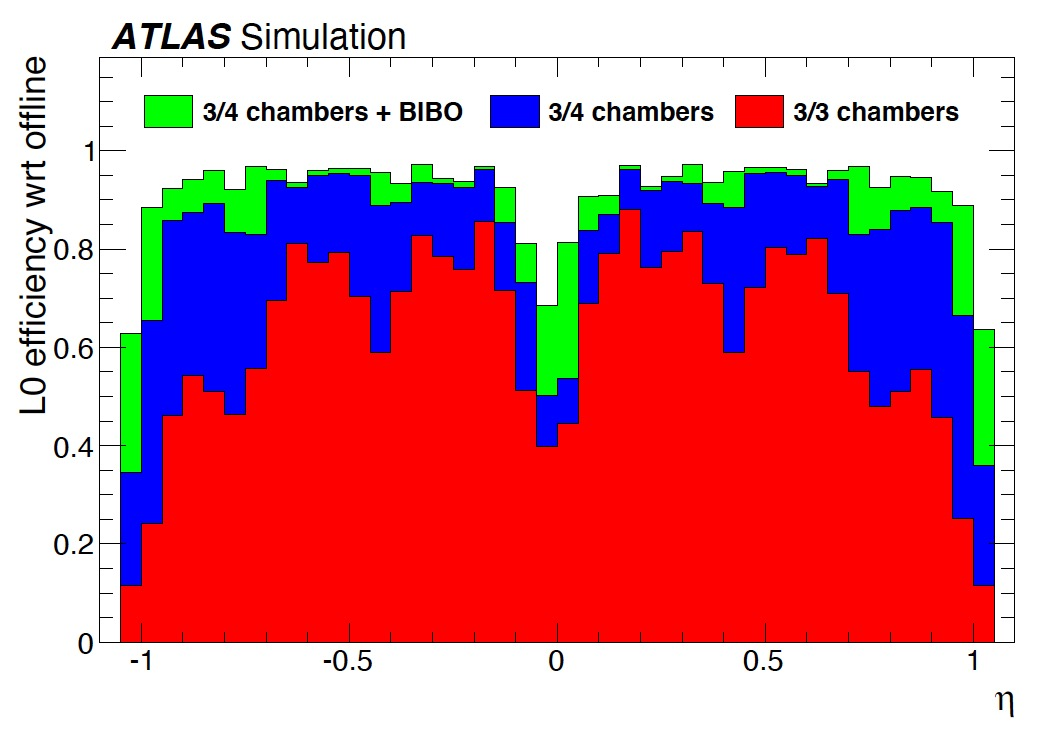
\includegraphics[width=0.9\textwidth]{Chapters/CH3/figures/tdr_eff}
	\caption{Efficiency times acceptance of the L0 barrel trigger for reconstructed muons with $p_{T} =
     25$ GeV as a function of $\eta$, assuming the worst-case scenario~\cite{TDR}.}
	\label{fig:tdr_eff}
\end{figure}
\\The new BI RPC chambers will have three sensitive gas gaps that are read out independently.
A majority logic requiring hits in at least two out of three planes provides high efficiency
while suppressing the rate of random coincidences due to uncorrelated hits from
photons and neutrons. This is necessary, for instance, to keep the rate of BI-BO coincidences
at an acceptable level.\\
A major re-design of the RPC technology started around the year 2010, mainly aiming at a
better rate capability and ageing behaviour. The new design is based on a reduced thickness
of the gas gaps (from 2 mm to 1 mm) and of the resistive electrodes (from 1.8 mm to
1 mm), and on the use of a new generation of low-noise high-sensitivity amplifiers. Using
these amplifiers, full efficiency can be achieved for a lower voltage across the gas gap, thus
transferring part of the amplification from the gas avalanche to the electronics. In this way,
the RPCs can be operated at a reduced charge per avalanche, reducing the detector current
and thus improving rate capability and ageing.\\
A detail view of the positions of the BI RPCs in ATLAS is shown in Figure~\ref{fig:xy_BIRPC}.
\begin{figure}[!h]
	\centering
	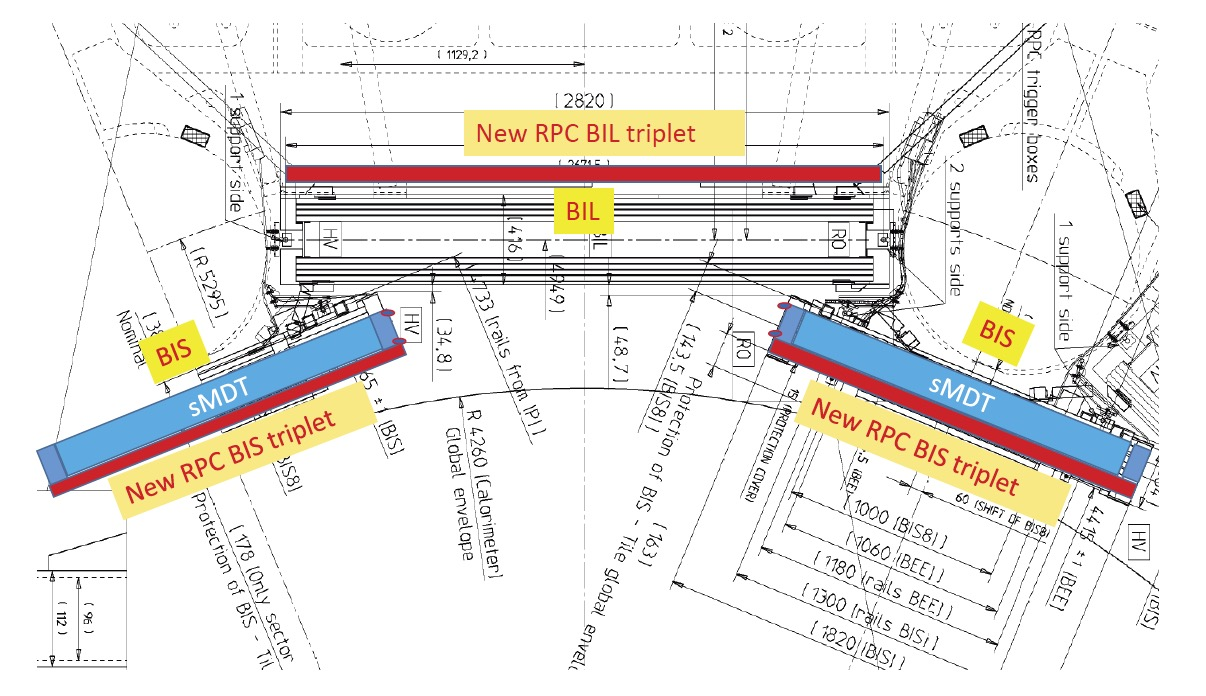
\includegraphics[width=0.9\textwidth]{Chapters/CH3/figures/xy_BIRPC}
	\caption{X-Y view of the inner barrel layer, indicating the positions of the BI RPCs (red) and BIS
sMDTs (blue) in the small and large sectors~\cite{TDR}.}
	\label{fig:xy_BIRPC}
\end{figure}
\\In the small sectors (BIS), due to the tight space limitations, the MDT chambers need to be 
replaced by new small-diameter MDT (sMDT) chambers with half the tube diameter (15 mm 
instead of 30 mm) in order to create space for the RPCs on the inside of the sMDT chambers. 
In  the large sectors (BIL), the new RPCs will be installed on the outside of the existing MDTs. The
layout of the new BI RPCs leaves the necessary holes and cut-outs for the existing MDT
alignment lines and for detector services. It comprises 272 triplet RPC chambers, for a total
area of about 470 $\mathrm{m^{2}}$. Acceptance studies based on a realistic description of the BI RPC geometry show a geometrical acceptance of the BI RPC chambers of 91$\%$ for reconstructed muons with $|\eta|$ < 1.05, compared to 95$\%$  for the MDT chambers. This results in a barrel trigger acceptance of 96$\%$.\\
Each detector layer of the triplets is read out on both surfaces by orthogonal strip panels,
providing $\eta$ and $\phi$ measurements. The compact triplet structure and the use of highly
sensitive amplifiers require a complete isolation of individual layers from each other. The
choice of strip pitches, 24–26 mm depending on the chamber type, has been constrained
by the performance requirements, the strip impedance, and cost considerations. The total
number of readout channels is about 8700.

\subsection {Trigger scheme}
\section{Hit digitization in the BI region}
\label{sec:trigScheme}
\clearpage
\subsection{Cluster Size model}

\clearpage
\subsection{Timing}

\clearpage
\subsection{BI RPCs with two-sides $\eta − \eta$ readout}
	
\clearpage
\section{L0 barrel trigger efficiency}

\clearpage
\subsection{BM and BO retrofitting}

\clearpage
\subsection{Dropping BIR and BIM chambers}

\clearpage
